\ifdefined\activerhandout 
\documentclass[12pt,aspectratio=1610,handout]{beamer}
\else
\documentclass[12pt,aspectratio=1610]{beamer}
\fi

%\usepackage[french]{babel} %=> erreur avec les tikz du moteur
\usepackage[T1]{fontenc}
\usepackage[utf8]{inputenc}
\usepackage{lmodern}
\usepackage{hyperref}
\usepackage{smartdiagram}
\usepackage{tikz}
\usepackage{animate}
\usepackage{tikzpeople}
\usepackage{appendixnumberbeamer}
\usepackage[labelformat=empty]{caption}
%\usepackage{pictochrono}
\usepackage{fontawesome5}
\usepackage{awesomebox}

\usetheme{Warsaw}
\setbeamertemplate{page number in head/foot}[totalframenumber]

\newcommand{\anglais}[1]{(\textit{\color{blue}#1})}
\newcommand{\legende}[2]{\caption[#1 (Source : \cite{#2})]{#1}}
\newcommand{\histoire}[1]{\begin{awesomeblock}{2pt}{\faBook}{black!75}#1\end{awesomeblock}}
\newcommand{\info}[1]{\begin{awesomeblock}{2pt}{\faInfoCircle}{black!75}#1\end{awesomeblock}}
\newcommand{\question}[1]{\begin{awesomeblock}{2pt}{\faQuestionCircle}{black!75}#1\end{awesomeblock}}
\newcommand{\alerte}[1]{\begin{awesomeblock}{2pt}{\faExclamationCircle}{black!75}#1\end{awesomeblock}}
\newcommand{\astuce}[1]{\begin{awesomeblock}{2pt}{\faLightbulb}{black!75}#1\end{awesomeblock}}
\newcommand{\exemple}[1]{\begin{awesomeblock}{2pt}{\faSearch}{black!75}#1\end{awesomeblock}}
\newcommand{\definitionAConnaitre}[1]{\begin{awesomeblock}{2pt}{\faCog}{black!75}#1\end{awesomeblock}}

\newcommand{\qmcBia}[7]{
%1 : titre slide
%2 : numéro de la bonne réponse
%3 : Inititulé de la question
%4, 5, 6, et 7 : propositions de réponse
\begin{frame}{#1}
\begin{awesomeblock}{2pt}{\faQuestion}{black!75}
#3
	\begin{enumerate}
	\ifnum#2=1
		\only<1>{\item #4}
		\only<2>{\item \textbf{#4}}
	\else
		\item #4
	\fi
	\ifnum#2=2
		\only<1>{\item #5}
		\only<2>{\item \textbf{#5}}
	\else
		\item #5
	\fi
	\ifnum#2=3
		\only<1>{\item #6}
		\only<2>{\item \textbf{#6}}
	\else
		\item #6
	\fi
	\ifnum#2=4
		\only<1>{\item #7}
		\only<2>{\item \textbf{#7}}
	\else
		\item #7
	\fi
	\end{enumerate}
	\pause
\end{awesomeblock}
\end{frame}
}

\subtitle{BIA - Brevet d'Initiation Aéronautique}
\author{Clément \textsc{Vermot-Desroches}}
\institute{Collège Aliénor d'Aquitaine\\Martignas-sur-Jalle}
\date{\today}

%\AtBeginSection[]
%{
%    \begin{frame}
%        %\frametitle{Table of Contents}
%        \tableofcontents[currentsection]
%    \end{frame}
%}

\AtBeginSubsection[]
{
    \begin{frame}
        %\frametitle{Table of Contents}
        \tableofcontents[currentsection,currentsubsection]
    \end{frame}
}
\input{commun/video.tex}

\addbibresource{01-EtudeAeronefs/biblio.bib}
\addbibresource{05-Histoire/biblio.bib}

\input{01-EtudeAeronefs/img/Cycle4Temps/ElementsMoteur.tex}

\title[Séance 2 - Constitution aérodyne]{Séance 2 \\ Structure avion \& Motorisation}

\usepackage{animate}

\begin{document}
 \begin{frame}
 \titlepage
 \end{frame}
 
 \begin{frame}
 \tableofcontents
 \end{frame}
 
 \section{La cellule d'un aéronef}
 \subsection{Vocabulaire}
 \begin{frame}{Description générale}
 \begin{figure}[H]
  	\only<1>{\includegraphics[scale=0.6]{01-EtudeAeronefs/img/celluleAvionNonLegendee.pdf}}
  	\only<2>{\includegraphics[scale=0.6]{01-EtudeAeronefs/img/celluleAvionLegendee.pdf}}
  	\pause
	\end{figure}
 \end{frame}
 
 \subsection{Différents dispositions de cellules}
 \begin{frame}{Différents types de train d'atterrissage}
 
 \begin{columns}
 \begin{column}{0.5\textwidth}
 \begin{figure}[H]
  		\centering
  		\includegraphics[width=0.95\textwidth,trim={0 2cm 0 2cm},clip]{01-EtudeAeronefs/img/D140.jpg}
  		\legende{Train classique}{img:D140}	
		\end{figure}
		\begin{itemize}
			\item disposition "historique"
			\item légèrement plus performant en vol
			\item roulage, décollage, atterrissage plus difficiles
		\end{itemize}
 \end{column}
 \begin{column}{0.5\textwidth}
 \begin{figure}[H]
  		\centering
  		\includegraphics[width=0.95\textwidth]{01-EtudeAeronefs/img/DR400.jpg}
  		\legende{Train tricycle}{img:DR400}	
		\end{figure}
		\begin{itemize}
			\item Protège l'hélice
			\item Meilleure visibilité au sol
		\end{itemize}
 \end{column}
 \end{columns}
 
 \end{frame} 
 
 \begin{frame}{Différentes configurations d'ailes : les multiplans}
 	Au début de l'aviation, on multiplie les ailes pour augmenter la portance et la rigidité. On parle de l'ère des multiplans (par opposition aux monoplans).
 	
 \begin{columns}
 \begin{column}{0.33\textwidth}
 \begin{figure}[H]
  		\centering
  		\includegraphics[width=0.95\textwidth]{01-EtudeAeronefs/img/ailes/Biplane_wire.pdf}
  		\legende{Biplan}{wing:Biplane-wire}	
		\end{figure}
 \end{column}
 \begin{column}{0.33\textwidth}
 \begin{figure}[H]
  		\centering
  		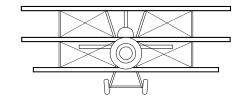
\includegraphics[width=0.95\textwidth]{01-EtudeAeronefs/img/ailes/Triplane.pdf}
  		\legende{Triplan}{wing:Triplane}	
		\end{figure}
 \end{column}
 \begin{column}{0.33\textwidth}
 \begin{figure}[H]
  		\centering
  		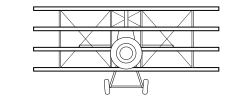
\includegraphics[width=0.95\textwidth]{01-EtudeAeronefs/img/ailes/Quadruplane.pdf}
  		\legende{Quadriplan}{wing:Quadruplane}	
		\end{figure}
 \end{column}
 \end{columns}
 
 \begin{columns}
 \begin{column}{0.33\textwidth}
 \begin{figure}[H]
  		\centering
  		\includegraphics[width=0.8\textwidth]{05-Histoire/img/wrightFlyer.jpg}
  		\legende{Le Wright Flyer}{img:wrightFlyer}	
		\end{figure}
 \end{column}
 \begin{column}{0.33\textwidth}
 \begin{figure}[H]
  		\centering
  		\includegraphics[width=0.8\textwidth]{05-Histoire/img/sopwithTriplane.jpg}
  		\legende{Sopwith Triplane}{img:sopwithTriplane}	
		\end{figure}
 \end{column}
 \begin{column}{0.33\textwidth}
 \begin{figure}[H]
  		\centering
  		\includegraphics[width=0.95\textwidth]{05-Histoire/img/bessonH5.jpg}
  		\legende{Besson H5}{img:bessonH5}	
		\end{figure}
 \end{column}
 \end{columns}
 
 \end{frame}
 
 \begin{frame}{Différentes configurations d'ailes : le dièdre}
	Le dièdre est l'angle formé par le plan de chaque aile et le plan horizontal. Il peut être positif, nul ou négatif. Le dièdre a un impact sur la stabilité.
 
 \begin{columns}
 \begin{column}{0.33\textwidth}
 \begin{figure}[H]
  		\centering
  		\includegraphics[width=0.95\textwidth]{01-EtudeAeronefs/img/ailes/Monoplane_dihedral.pdf}
  		\legende{Dièdre positif}{wing:Monoplane-dihedral}	
		\end{figure}
 \end{column}
 \begin{column}{0.33\textwidth}
 \begin{figure}[H]
  		\centering
  		\includegraphics[width=0.95\textwidth]{01-EtudeAeronefs/img/ailes/Monoplane_mid.pdf}
  		\legende{Dièdre nul}{wing:Monoplane-mid}	
		\end{figure}
 \end{column}
 \begin{column}{0.33\textwidth}
 \begin{figure}[H]
  		\centering
  		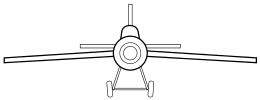
\includegraphics[width=0.95\textwidth]{01-EtudeAeronefs/img/ailes/Monoplane_anhedral.pdf}
  		\legende{Dièdre négatif}{wing:Monoplane-anhedral}	
		\end{figure}
 \end{column}
 \end{columns}
 
 \end{frame}
 
 \begin{frame}{Différentes configurations d'ailes : différentes configurations}
	Il existe de nombreuses formes d'ailes. En voici quelques unes.
 
 \begin{columns}
 \begin{column}{0.33\textwidth}
 \begin{figure}[H]
  		\centering
  		\includegraphics[width=0.95\textwidth]{01-EtudeAeronefs/img/ailes/Wing_constant.pdf}
  		\legende{Aile rectangulaire}{wing:Wing-constant}	
		\end{figure}
 \end{column}
 \begin{column}{0.33\textwidth}
 \begin{figure}[H]
  		\centering
  		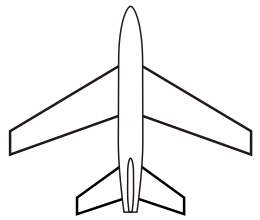
\includegraphics[width=0.95\textwidth]{01-EtudeAeronefs/img/ailes/Wing_swept.pdf}
  		\legende{Aile en flèche}{wing:Wing-swept}	
		\end{figure}
 \end{column}
 \begin{column}{0.33\textwidth}
 \begin{figure}[H]
  		\centering
  		\includegraphics[width=0.95\textwidth]{01-EtudeAeronefs/img/ailes/Wing_elliptical.pdf}
  		\legende{Aile elliptique}{wing:Wing-elliptical}	
		\end{figure}
 \end{column}
 \end{columns}
 \end{frame}
 
 \begin{frame}{Différentes configurations d'ailes : différentes configurations}
	Il existe de nombreuses formes d'ailes. En voici quelques unes.
 
 \begin{columns}
 \begin{column}{0.33\textwidth}
 \begin{figure}[H]
  		\centering
  		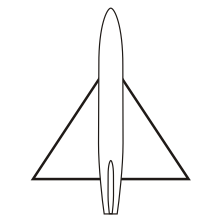
\includegraphics[width=0.95\textwidth]{01-EtudeAeronefs/img/ailes/Wing_tailless_delta.pdf}
  		\legende{Aile delta}{wing:Wing-tailless-delta}	
		\end{figure}
 \end{column}
 \begin{column}{0.33\textwidth}
 \begin{figure}[H]
  		\centering
  		\includegraphics[width=0.95\textwidth]{01-EtudeAeronefs/img/ailes/Wing_ogival_delta.pdf}
  		\legende{Aile gothique}{wing:Wing-ogival-delta}	
		\end{figure}
 \end{column}
 \begin{column}{0.33\textwidth}
 \begin{figure}[H]
  		\centering
  		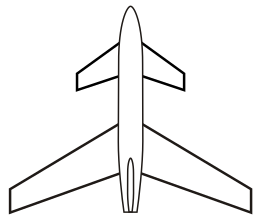
\includegraphics[width=0.95\textwidth]{01-EtudeAeronefs/img/ailes/Wing_canard.pdf}
  		\legende{Configuration canard}{wing:Wing-canard}	
		\end{figure}
 \end{column}
 \end{columns}
 \end{frame}
 
 \begin{frame}{Différentes configurations d'ailes : différentes configurations}
	Il existe de nombreuses formes d'ailes. En voici quelques unes.
 
 \begin{columns}
 \begin{column}{0.33\textwidth}
 \begin{figure}[H]
  		\centering
  		\includegraphics[width=0.95\textwidth]{01-EtudeAeronefs/img/mirage2000.jpg}
  		\legende{Aile delta : chasseur}{img:mirage2000}	
		\end{figure}
 \end{column}
 \begin{column}{0.33\textwidth}
 \begin{figure}[H]
  		\centering
  		\includegraphics[width=0.95\textwidth]{01-EtudeAeronefs/img/concorde.jpg}
  		\legende{Aile gothique : Concorde}{img:concorde}	
		\end{figure}
 \end{column}
 \begin{column}{0.33\textwidth}
 \begin{figure}[H]
  		\centering
  		\includegraphics[width=0.95\textwidth]{01-EtudeAeronefs/img/rutanLongEz.jpg}
  		\legende{Canard : Long EZ}{img:rutanLongEz}	
		\end{figure}
 \end{column}
 \end{columns}
 \end{frame}
 
 \section{Le moteur 4 temps}
 \begin{frame}{Le moteur à combustion interne}
	\begin{figure}[H]
  	\only<1>{\includegraphics[scale=0.7]{01-EtudeAeronefs/img/Cycle4Temps/0-MoteurLegendeFlechesSeulement_doc.pdf}}
  	\only<2>{\includegraphics[scale=0.7]{01-EtudeAeronefs/img/Cycle4Temps/0-MoteurLegende_doc.pdf}}
	\end{figure}
	\pause
 \end{frame}
 
 \subsection{Le cycle à 4 temps}
 \begin{frame}{Admission}
 \begin{columns}
 \begin{column}{0.65\textwidth}
 	\only<2>{\begin{itemize}
 		\item La soupape d'admission est ouverte
 		\item Le piston descend
 		\item Le mélange air-carburant est aspiré dans le cylindre
 	\end{itemize}}
 \end{column}
 \begin{column}{0.35\textwidth}
 \begin{figure}[H]
  		\centering
  		\renewcommand{\echelleTikz}{0.5}
  		\scalebox{1.2}{\begin{minipage}{3cm}
		% INTAKE STROKE
\def\gas{blue!50}
\begin{tikzpicture}[scale=\echelleTikz]
  \def\d{-60}
  \engine{10};
  %\draw[vector] (\d:.6*\R) arc (\d:\d-80:.55*\R);
  \fill[\gas, opacity=0.5]
    (VLo) to[out=110,in=0] ++ (-1.5,0.6) -- ($(VLo)+(-1.5,1.3)$) to[out=0,in=110] (VLm) to[out=\vl+5,in=\vl-47] cycle;
  \wall
  \valveL{.3}
  \valveR{.1};
  
\end{tikzpicture}
		\end{minipage}	}	
		\end{figure}
 \end{column}
 \end{columns}
 \pause
 \end{frame} 
 
 \begin{frame}{Compression}
 \begin{columns}
 \begin{column}{0.35\textwidth}
 \begin{figure}[H]
  		\centering
  		\renewcommand{\echelleTikz}{0.5}
  		\scalebox{1.2}{\begin{minipage}{3cm}
		% COMPRESSION STROKE
\begin{tikzpicture}[scale=\echelleTikz]
  \def\d{-10}
  \engine{-140};
  \draw[vector] (\d:.6*\R) arc (\d:\d-80:.55*\R);
  \valveL{.1}
  \valveR{.1}
\end{tikzpicture}
		\end{minipage}	}	
		\end{figure}
 \end{column}
 \begin{column}{0.65\textwidth}
 	\only<2>{\begin{itemize}
 		\item Les soupapes sont fermées
 		\item Le piston remonte
 		\item Le mélange est compressé dans le cylindre.
 	\end{itemize}}
 \end{column}
 \end{columns}
 \pause
 \end{frame} 
 
  \begin{frame}{Explosion-détente}
 \begin{columns}
 \begin{column}{0.65\textwidth}
 	\only<2-4>{\begin{itemize}
 		\item Les soupapes sont fermées
 		\item La bougie produit une étincelle quand le piston est au point haut
 		\item Le piston est repoussé vers le bas par l'explosion
 	\end{itemize}
 	\only<3-4>{\info{Le temps d'explosion-détente est le seul temps qui produit de l'énergie}}
 	\only<4>{\alerte{Un moteur d'avion est généralement équipé de 2 bougies par cylindre pour augmenter la sécurité}}}
 \end{column}
 \begin{column}{0.35\textwidth}
 \begin{figure}[H]
  		\centering
  		\renewcommand{\echelleTikz}{0.5}
  		\scalebox{1.2}{\begin{minipage}{3cm}
		% IGNITION
\begin{tikzpicture}[scale=\echelleTikz]
  \def\d{40}
  \engine{90};
  \draw[vector] (\d:.6*\R) arc (\d:\d-80:.55*\R);
  \valveL{.1}
  \valveR{.1}
  \draw[very thin,yellow!70!black,fill=yellow,shift={(X)}]
    ( -15:.20) -- ( -30:.40) -- ( -40:.25) -- ( -50:.40) --
    ( -60:.22) -- ( -70:.40) -- ( -80:.20) -- ( -90:.45) --
    (-100:.24) -- (-110:.40) -- (-120:.25) -- (-130:.40) --
    (-140:.20) -- (-150:.45) -- (-165:.20) to[out=40,in=140] cycle;
\end{tikzpicture}
		\end{minipage}	}	
		\end{figure}
 \end{column}
 \end{columns}
 \pause
 \pause
 \pause
 \end{frame} 
 
 \begin{frame}{Échappement}
 \begin{columns}
 \begin{column}{0.35\textwidth}
 \begin{figure}[H]
  		\centering
  		\renewcommand{\echelleTikz}{0.5}
  		\scalebox{1.2}{\begin{minipage}{3cm}
		% EXHAUST STROKE
\def\gas{blue!50}
\begin{tikzpicture}[scale=\echelleTikz]
  \def\d{-40}
  \engine{-190};
  \draw[vector] (\d:.6*\R) arc (\d:\d-80:.55*\R);
  \fill[\gas, opacity=0.5]
    (VRo) to[out=60,in=-180] ++ (1.5,0.6) -- ($(VRo)+(1.5,1.3)$) to[out=180,in=60] (VRm) to[out=-220+\vr,in=-180+\vr] cycle;
  \wall
  \valveL{.1}
  \valveR{.3}
\end{tikzpicture}
		\end{minipage}	}	
		\end{figure}
 \end{column}
 \begin{column}{0.65\textwidth}
 	\only<2>{\begin{itemize}
 		\item La soupape d'échappement s'ouvre
 		\item La remontée du piston chasse les gaz brulés du cylindre
 	\end{itemize}}
 \end{column}
 \end{columns}
 \pause
 \end{frame}
 
 \begin{frame}{Cycle complet}
 \begin{figure}[H]
  		\centering
  		\renewcommand{\echelleTikz}{0.5}
  		\scalebox{.6}{\begin{minipage}{3cm}
		% Définition des couleurs de base
\definecolor{gazFroid}{RGB}{173,216,230}     % Bleu clair
\definecolor{gazChaud}{RGB}{255,0,0}         % Rouge
\definecolor{gazExplosion}{RGB}{255,255,0}   % Jaune
\definecolor{gazBrule}{RGB}{128,128,128}     % Gris

% Définition des couleurs de base
\definecolor{gazFroid}{RGB}{173,216,230}     % Bleu clair
\definecolor{gazChaud}{RGB}{255,0,0}         % Rouge
\definecolor{gazExplosion}{RGB}{255,255,0}   % Jaune
\definecolor{gazBrule}{RGB}{128,128,128}     % Gris

% Définition de la couleur des gaz en fonction de l'angle
\newcommand{\setGasColor}[1]{%
    \def\angle{#1}%
    % De gris à bleu (-90 à -30)
    \ifnum\angle<-30
        \def\gas{gazBrule!\the\numexpr100-(((\angle+90)*100)/60)\relax!gazFroid}%
    \else
        % Bleu constant (-30 à 90)
        \ifnum\angle<90
            \def\gas{gazFroid}%
        \else
            % De bleu vers rouge (90 à 270)
            \ifnum\angle<270
                \def\gas{gazFroid!\the\numexpr100-((\angle-90)*100/180)\relax!gazChaud}%
            \else
                % De rouge vers jaune (270 à 300)
                \ifnum\angle<300
                    \def\gas{gazChaud!\the\numexpr((\angle-270)*100/30)\relax!gazExplosion}%
                \else
                    % De jaune vers gris (300 à 450)
                    \ifnum\angle<450
                        \def\gas{gazExplosion!\the\numexpr100-((\angle-300)*100/150)\relax!gazBrule}%
                    \else
                        % Gris constant (450 à 630)
                        \def\gas{gazBrule}%
                    \fi
                \fi
            \fi
        \fi
    \fi
}

\ifdefined\activeranimations 
\newcommand{\nbFramesMoteurAnime}{360}
\else
\newcommand{\nbFramesMoteurAnime}{1}
\fi

\begin{animateinline}[autoplay,loop,controls]{60}
\multiframe{\nbFramesMoteurAnime}{i=-90+2}{%
    \begin{tikzpicture}
    \setGasColor{\i}%
      \coordinate (boiteLegende1) at (0,8.5);
      \coordinate (boiteLegende2) at (0,9);
      \node[rectangle,minimum width=2cm] [fit = (boiteLegende1) (boiteLegende2)] (legende) {};    
    
      \engine{-\i}
      
      % INTAKE STROKE
      \ifnum\i>-92 \ifnum\i<-88 
          \node[align=center,font=\Large] at (legende.center) {\textbf{Admission}};
          \valveL{.2}
          \valveR{.1};
      \fi \fi 
      \ifnum\i>-90 \ifnum\i<90 
          \node[align=center,font=\Large] at (legende.center) {\textbf{Admission}};
          \setGasColor{\i}%
          \fill[\gas, opacity=0.5]
              (VLo) to[out=110,in=0] ++ (-1.5,0.6) -- ($(VLo)+(-1.5,1.3)$) to[out=0,in=110] (VLm) to[out=\vl+5,in=\vl-47] cycle;
          \wall
          \valveL{.3}
          \valveR{.1};
      \fi \fi
      
      % COMPRESSION STROKE
      \ifnum\i>90 \ifnum\i<272 
          \node[align=center,font=\Large] at (legende.center) {\textbf{Compression}};
          \valveL{.1}
          \valveR{.1};
      \fi \fi 
      
      % POWER STROKE
      \ifnum\i>270 \ifnum\i<452 
          \node[align=center,font=\Large] at (legende.center) {\textbf{Explosion-détente}};
          \valveL{.1}
          \valveR{.1};
      \fi \fi
      
      % EXHAUST STROKE
      \ifnum\i>452 \ifnum\i<630
          \node[align=center,font=\Large] at (legende.center) {\textbf{Echappement}};
          \fill[\gas, opacity=0.5]
              (VRo) to[out=60,in=-180] ++ (1.5,0.6) -- ($(VRo)+(1.5,1.3)$) to[out=180,in=60] (VRm) to[out=-220+\vr,in=-180+\vr] cycle;
          \wall 
          \valveL{.1}
          \valveR{.3};
      \fi \fi
      
      % IGNITION
      \ifnum\i>268 \ifnum\i<280 
          \draw[very thin,yellow!70!black,fill=yellow,shift={(X)}]
              ( -15:.20) -- ( -30:.40) -- ( -40:.25) -- ( -50:.40) --
              ( -60:.22) -- ( -70:.40) -- ( -80:.20) -- ( -90:.45) --
              (-100:.24) -- (-110:.40) -- (-120:.25) -- (-130:.40) --
              (-140:.20) -- (-150:.45) -- (-165:.20) to[out=40,in=140] cycle; 
      \fi \fi 
    \end{tikzpicture}
  }
\end{animateinline}
		\end{minipage}	}	
		\end{figure}		
 \end{frame}
 
 \begin{frame}{Système d'allumage}
 \begin{columns}
 \begin{column}{0.5\textwidth}
 	\begin{itemize}
 		\item Double magnéto : améliore la fiabilité
 		\item Double bougie : améliore la combustion
 		\item Sélecteur de magnéto dans le cockpit
 	\end{itemize}
 \end{column}
 \begin{column}{0.5\textwidth}
 	\begin{figure}[H]
  		\centering
    		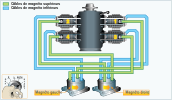
\includegraphics[width=1.07\textwidth]{01-EtudeAeronefs/img/systemesAvion/systemeAllumage.pdf}
  		\legende{Système d'allumage}{img:systemeAllumage}
	\end{figure}	
 \end{column}
 \end{columns}
 \end{frame}
 
 \begin{frame}{Carburateur}
 \begin{columns}
 \begin{column}{0.5\textwidth}
 	\begin{itemize}
 		\item Produit le mélange air-carburant ($1/15^{ième}$)
 		\item Dépression dans le venturi
 		\only<2>{\item Givrage carburateur}
 	\end{itemize}
 	\only<2>{\begin{figure}[H]
  		\centering
    		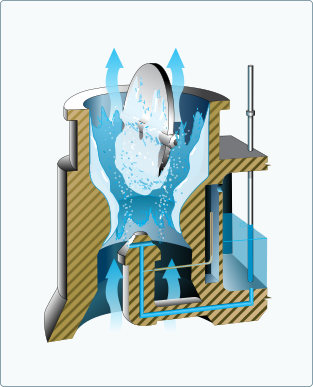
\includegraphics[width=0.5\textwidth]{01-EtudeAeronefs/img/systemesAvion/givrageCarbu.pdf}
  		\legende{Givrage carbu}{img:givrageCarbu}
	\end{figure}	}
 \end{column}
 \begin{column}{0.5\textwidth}
 	\begin{figure}[H]
  		\centering
    		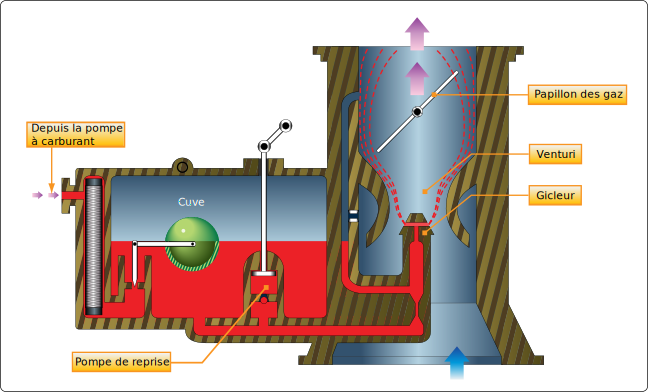
\includegraphics[width=1.07\textwidth]{01-EtudeAeronefs/img/systemesAvion/carburateur.pdf}
  		\legende{Schéma d'un carburateur}{img:carburateur}
	\end{figure}	
 \end{column}
 \end{columns}
 
 \pause
 \end{frame}
 
 \subsection{Différentes dispositions de cylindres}
 \begin{frame}{Les dispositions de cylindres}
 Afin d'augmenter la puissance des moteurs et d'améliorer la régularité de fonctionnement, les concepteurs des moteurs ont rapidement multiplié le nombre de cylindres de leurs moteurs.
 
 \question{Connaissez vous des dispositions de cylindres ?}
 
 \end{frame}
 
 \begin{frame}{Les principales dispositions de cylindres - moteur en ligne}
 \begin{columns}
 \begin{column}{0.5\textwidth}
 	\begin{itemize}
 		\item Disposition simple
 		\item Refroidissement limité des cylindres du fond
 	\end{itemize}
 \end{column}
 \begin{column}{0.5\textwidth}
 	\begin{figure}[H]
  		\centering
    		\includegraphics[width=0.95\textwidth]{01-EtudeAeronefs/img/renault4P.png}
  		\legende{Moteur en ligne Renault 4P}{img:renault4P}
	\end{figure}	
 \end{column}
 \end{columns}
 \end{frame}
 
 \begin{frame}{Les principales dispositions de cylindres - moteur en ligne}
	\begin{figure}[H]
  	\scalebox{.3}{\embedvideo*{\includegraphics[page=1, scale=1]{01-EtudeAeronefs/img/flat4}}{01-EtudeAeronefs/img/video/flat4.mp4}}
  	\legende{Moteur en ligne 4 cylindres}{video:flat4}
	\end{figure}
\end{frame}
 
 \begin{frame}{Les principales dispositions de cylindres - moteur à plat}
 \begin{columns}
 \begin{column}{0.5\textwidth}
 	\begin{itemize}
 		\item Meilleur refroidissement
 		\item Moteur "plat" permettant une meilleure visibilité
 	\end{itemize}
 \end{column}
 \begin{column}{0.5\textwidth}
 	\begin{figure}[H]
  		\centering
    		\includegraphics[width=0.95\textwidth]{01-EtudeAeronefs/img/boxer6.jpg}
  		\legende{Moteur à plat 6 cylindres}{img:boxer6}
	\end{figure}	
 \end{column}
 \end{columns}
 \end{frame}

\begin{frame}{Les principales dispositions de cylindres - moteur à plat}
	\begin{figure}[H]
  	\scalebox{.3}{\embedvideo*{\includegraphics[page=1, scale=1]{01-EtudeAeronefs/img/boxer4}}{01-EtudeAeronefs/img/video/boxer4.mp4}}
  	\legende{Moteur à plat 4 cylindres}{video:boxer4}
	\end{figure}
\end{frame}

\begin{frame}{Les principales dispositions de cylindres - moteur en V}
 \begin{columns}
 \begin{column}{0.5\textwidth}
 	\begin{itemize}
 		\item plus court et plus léger qu'un moteur en ligne équivalent
 		\item Moins de vibrations
 	\end{itemize}
 \end{column}
 \begin{column}{0.5\textwidth}
 	\begin{figure}[H]
  		\centering
    		\includegraphics[width=0.95\textwidth]{01-EtudeAeronefs/img/moteurV12.jpg}
  		\legende{Moteur V12}{img:moteurV12}
	\end{figure}	
 \end{column}
 \end{columns}
 \end{frame}
 
 \begin{frame}{Les principales dispositions de cylindres - moteur en V}
	\begin{figure}[H]
  	\scalebox{.3}{\embedvideo*{\includegraphics[page=1, scale=1]{01-EtudeAeronefs/img/v6}}{01-EtudeAeronefs/img/video/v6.mp4}}
  	\legende{Moteur V6}{video:v6}
	\end{figure}
\end{frame}

\begin{frame}{Les principales dispositions de cylindres - étoile}
 \begin{columns}
 \begin{column}{0.5\textwidth}
 	\begin{itemize}
 		\item Compact, léger, peu couteux
 		\item Système de graissage adapté au vol acrobatique
 		\item Refroidissement optimum
 	\end{itemize}
 \end{column}
 \begin{column}{0.5\textwidth}
 	\begin{figure}[H]
  		\centering
    		\includegraphics[width=0.95\textwidth]{01-EtudeAeronefs/img/PWWasp.jpg}
  		\legende{Moteur en étoile P\& W Wasp}{img:PWWasp}
	\end{figure}	
 \end{column}
 \end{columns}
 \end{frame}

\begin{frame}{Les principales dispositions de cylindres - étoile}
 \begin{figure}[H]
  	\scalebox{.3}{\embedvideo*{\includegraphics[page=1, scale=1]{01-EtudeAeronefs/img/9cylindresEtoile}}{01-EtudeAeronefs/img/video/9cylindresEtoile.mp4}}
  	\legende{Moteur en étoile 9 cylindres}{video:9CylindresEtoile}
	\end{figure}
	\end{frame}
 
\appendix 
\section{QCM}
 \qmcBia{Étude des aéronefs}
{3}{Dans un moteur à 4 temps, la compression intervient après :}
{la combustion}
{la détente}
{l'admission}
{l'échappement}

 \qmcBia{Étude des aéronefs}
{2}{Durant un cycle de fonctionnement d'un moteur à pistons (4 temps), le seul temps où le piston monte du point mort bas au point mort haut avec les soupapes fermées est le temps :}
{d'admission}
{de compression}
{de combustion-détente}
{d'échappement}

\qmcBia{Étude des aéronefs}
{3}{Sur un avion certifié, un moteur à pistons contenant 4 cylindres est pourvu au total de :}
{2 bougies d'allumage}
{4 bougies d'allumage}
{8 bougies d'allumage}
{0 bougie d'allumage}

\qmcBia{Étude des aéronefs}
{3}{\begin{figure}[H]
  		\centering
    		\includegraphics[width=0.2\textwidth]{01-EtudeAeronefs/img/PWWasp.jpg}
	\end{figure}	
	La disposition des cylindres de ce moteur est :}
{en ligne}
{en V}
{en étoile}
{à plat} 
 
\ifdefined\activerbibliobeamer
\begin{frame}[allowframebreaks]
\frametitle{Bibliographie}
\printbibliography
%\nocite{*}
\end{frame}
\fi 
 
\end{document}
